\documentclass[4:3]{lecture}
\usepackage{amsmath,amssymb,inconsolata,relsize,bm,xcolor,hyperref,multicol,booktabs,suffix}
\usepackage[fixed]{fontawesome5} 

% Colors
\definecolor{backgroundlightgray}{gray}{0.97}
\colorlet{hidden}{mediumgray}
\definecolor{fsublue}{RGB}{0,47,93}

% Macros
\newcommand{\query}[1]{\textbf{{\texttt{\smaller #1}}}\xspace}

\let\item\itemaux
\newcommand{\faItem}[1]{\item[\smaller\faIcon{#1}\hspace*{-0.4em}]}
\WithSuffix\newcommand\faItem*[1]{\item[\smaller\smaller\raisebox{0.1ex}{\faIcon{#1}}\hspace*{-0.4em}]}

\newcommand{\paperTitle}{How does search engine result quality impact our decisions?}
\bsauthor{Heinrich, Lena, Sascha}
\bsyear{2024}

\begin{document}

\pagestyle{empty}

\begin{bsslide}
  \begin{center}
    \hfill\vfill 
    {\large How does search engine result quality impact our decisions?}
    {\color{fsublue}\rule{\textwidth}{1.5pt}}
    \vspace*{0.25ex}
    Heinrich \hspace{4em} Lena \hspace{4em} Sascha
    \vspace*{1ex}
    \begin{center}
      \vspace{2ex}
      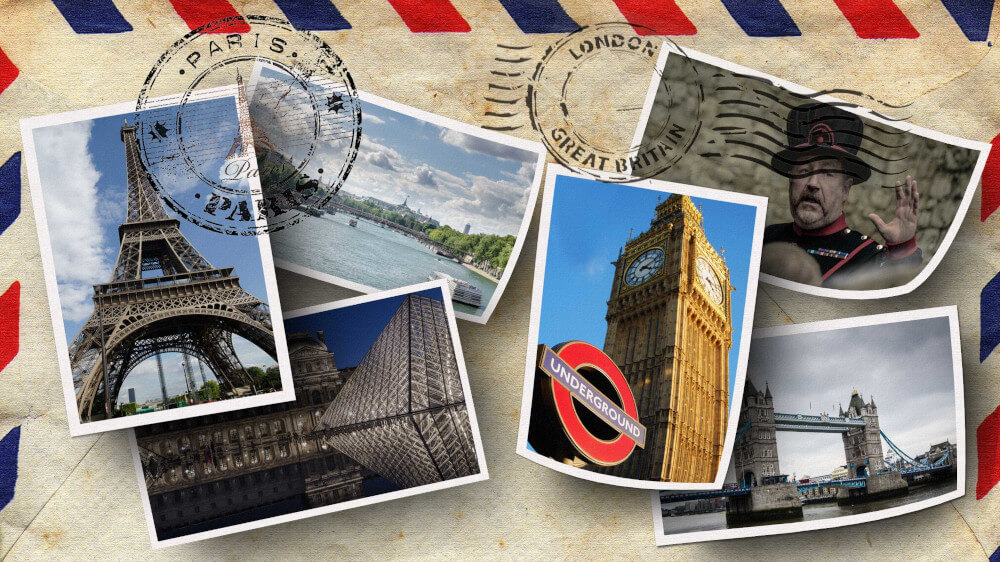
\includegraphics[width=0.65\linewidth]{paris-vs-london}\\[-1.5ex]
      {\tiny Source: \url{https://netivist.org/debate/paris-vs-london}}\\[1ex]
      \raisebox{0.2ex}{\textcolor{gray}{\small Thinking of}}
      {\large \faIcon{comment-dots} Which city is better, Paris or London?}
      \phantom{{\small Thinking of}}
    \end{center}
    \vfill
  \end{center}
\end{bsslide}

\pagestyle{plain}

\colorlet{colorA}{hidden}
\colorlet{colorB}{webisblueLD!50!white}
\newcommand{\memeGoogle}{meme-google-gray}
\begin{bsslide}[\paperTitle]
  \vspace*{1ex}
  \begin{minipage}[t]{0.55\linewidth}
    \begin{center}
      \colortext{\faIcon{exchange-alt} Ideally..}
    \end{center}
    Should use an \emph{argument} search engine. \\
    \begin{itemize}
      \faItem{arrow-right} Consider relevance \emph{and} quality \\
      \textcolor{gray}{e.g., args.me or ArgumenText}
    \end{itemize}
    \begin{center}
      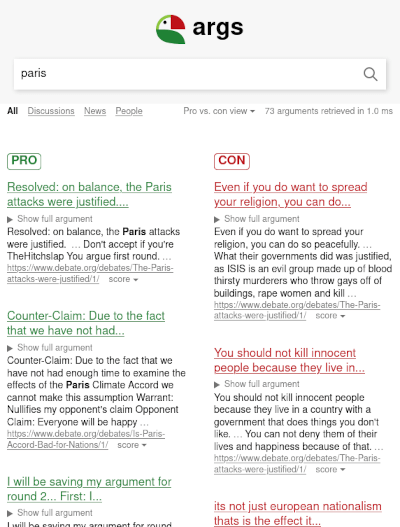
\includegraphics[width=0.5\linewidth]{screenshot-argsme}      
    \end{center}
    \begin{itemize}
      \faItem{arrow-right} Not (yet) fit for \emph{comparative} topics
    \end{itemize}
  \end{minipage}
  \hspace{1.2em}
  \begin{minipage}[t]{0.4\linewidth}
    \begin{center}
      \colortext[colorB]{\faIcon{compass} But..}
    \end{center}
    \color{colorA}Nah, just ``google'' it! \\[2ex]
    \begin{center}
      \includegraphics[width=1\linewidth]{\memeGoogle}      
    \end{center}
  \end{minipage}
\end{bsslide}
\colorlet{colorA}{black}
\colorlet{colorB}{webisblueLD}
\renewcommand{\memeGoogle}{meme-google}
\begin{bsslide}[\paperTitle]
  \lastslide
\end{bsslide}

\colorlet{colorA}{hidden}
\newcommand{\memeThinking}{meme-thinking-gray}
\begin{bsslide}[\paperTitle]
  \colortext{Our experiments}
  \vspace{1ex}
  \begin{center}
    ``Paris vs.\ London? How would you decide, given Google's top results?''
  \end{center}
  \vspace{1.5ex}
  \begin{minipage}[c]{0.59\linewidth}
    \begin{enumerate}
      \setlength{\itemsep}{1.25ex}
      \item Select 30~comparative questions (Touché)
      \item Assess \emph{quality} of 120~top Google results
      \begin{itemize}
        \setlength{\itemsep}{0.5ex}
        \faItem{file-alt} Content quality
        \faItem{universal-access} Usability
        \faItem{shield-alt} Credibility
        \faItem{stopwatch} Up-to-dateness
      \end{itemize}
      \item User study on \emph{decision-making}
      \begin{itemize}
        \setlength{\itemsep}{0.5ex}
        \faItem{random} Decision change
        \faItem{compass} Decision confidence (+ conf.\ change)
        \faItem{exclamation-circle} Most impactful documents
        \faItem{comments} General decision-making process
      \end{itemize}
    \end{enumerate}
  \end{minipage}
  \hfill
  \color{colorA}
  {\Large\faIcon{caret-right}}
  \hfill
  \begin{minipage}[c]{0.33\linewidth}
    4. \emph{Analyze} reponses
    \begin{itemize}
      \item 554 study responses
      \item 8 compar.\ questions
      \item 6 hypotheses
      \faItem{arrow-right} verify with \(\chi^2\)~tests
    \end{itemize}
    \begin{center}
      \includegraphics[width=0.8\linewidth]{\memeThinking}
    \end{center}
  \end{minipage}
\end{bsslide}
\colorlet{colorA}{black}
\renewcommand{\memeThinking}{meme-thinking}
\begin{bsslide}[\paperTitle]
  \lastslide
\end{bsslide}

\colorlet{colorA}{white}
\begin{bsslide}[\paperTitle]
  \colortext{Results}
  \begin{center}
    
\includegraphics[width=0.7\linewidth]{meme-results}
  \end{center}
  \begin{itemize}
    \setlength{\itemsep}{1.75ex}
    \item High-quality search results are \emph{more likely} to influence decisions \\
    \textcolor{darkgray}{(users with high initial confidence less likely influenced by low-quality results)}
    \item Relevance and quality have \emph{similarly} strong impact on decision-making \\
    \textcolor{darkgray}{(impact of stance is weaker)}
    \item Factual comparisons \emph{more likely} influenced by search than subjective comp.
    \faItem*{clock} Future work: how to retrieve higher-quality search results?
  \end{itemize}
  \vfill
  \color{colorA}
  \begin{flushright}
    \large
    \emph{Thank you!}\vspace*{0.25ex}
  \end{flushright}
\end{bsslide}

\colorlet{colorA}{black}
\begin{bsslide}[\paperTitle]
    \lastslide
\end{bsslide}

\end{document}
